\textbf{Цель работы:} с помощью сцинтилляционного счётчика измеряются линейные коэффициенты ослабления потока $\gamma$-лучей в свинце, железе и алюминии; 
по их величине определяются энергия $\gamma$-квантов.

\textbf{В работе используются:} сцинтилляционный счётчик, образцы из свинца, железа и алюминия.
                    
\section{Теоретическое введение}

    $\gamma$-лучи возникают при переходе возбужденных ядер из одного энергетического состояния в другое, более низкое. Энергия $\gamma$-квантов обычно заключена между несколькими десятками килоэлектронвольт и несколькими миллионами электрон-вольт. Гамма-кванты не несут электрического заряда, их масса равна нулю. Проходя, через вещество, пучок $\gamma$-квантов постепенно ослабляется. Ослабление происходит по экспоненциальному закону, который может быть записан в следующих формах:
    \begin{equation}
        \label{I(mu)}
        I = I_0 e^{-\mu l}, \; I = I_0 e^{-\mu' m_1},
    \end{equation}
    где $I$, $I_0$ -- интенсивности прошедшего и падающего излучений; $l$ -- длина пути, пройденного пучком $\gamma$-лучей; $m_1$ - масса, пройденного вещества, приходящиеся на единицу площади; $\mu$ и $\mu'$ -- коэффициенты ослабления потока в веществе.

    Ослабление потока $\gamma$-лучей, происходящее при прохождении среды, связано с тремя эффектами: фотоэлектрическим поглощением, комптоновским рассеянием и с генерацией электрон-позитронных пар. Рассмотрим эти эффекты.

\subsection*{Фотоэлектрическое поглощение}

    При столкновении $\gamma$-квантов с электронами внутренних атомных оболочек может происходить поглощение квантов. Энергия $\gamma$-кванта передается соответствующему электрону, а импульс делится между этим электроном и оставшимся после его вылета ионом. Свободный электрон не может поглотить $\gamma$-квант, так как при этом невозможно одновременно удовлетворить законам сохранения энергии и импульса. Наружные электроны не принимают участия в фотоэлектрическом поглощении, потому что они слабо связаны в атоме, так что их практически можно считать свободными. Вероятность $dP_{\text{ф}}$ фотоэлектрического поглощения $\gamma$-квантов пропорциональна длине пути $dl$ и плотности электронов в среде (в расчет должны приниматься только электроны, принадлежащие внутренним оболочкам атомов):
	
	\begin{equation}
        \label{mu_ph}
	    dP_{\text{ф}} = \sigma_{\text{ф}} n_1 dl, \quad \mu_{\text{ф}} = \sigma_{\text{ф}} n_1
	\end{equation}
	
	Здесь $n_1$ -- плотность внутренних электронов, а $\sigma_{\text{ф}}$ -- поперечное сечение фотоэлектрического поглощения. Поперечное сечение характеризует вероятность фотоэффекта, рассчитанную на один электрон. Связь между $\mu_{\text{ф}}$ и $\sigma_{\text{ф}}$ устанавливается из формулы \eqref{I(mu)} и в явном виде определяет зависимости $\mu$ от плотности среды.
	
	Пусть в результате фотоэффекта энергия $\gamma$-кванта передается электрону, находящемуся на $i$-й оболочке атома. Обозначим через $W_i$
	энергию связи этого электрона. После вылета из атома электрон приобретает кинетическую энергию $T_i = \hbar \omega - W_i$. Освободившееся после вылета электрона место заполняется затем одним из электронов с вышележащих оболочек. При таких переходах возникает характеристическое рентгеновское излучение.

    \begin{figure}[h!]
        \centering
        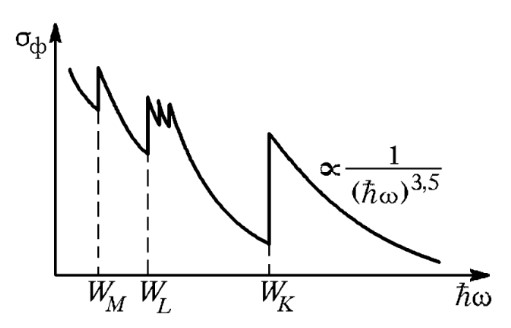
\includegraphics[width = 8 cm]{images/photo_effect}
        \caption{Зависимость сечения фотоэффекта от энергии $\gamma$-квантов}
        \label{photo_effect}
    \end{figure}
	
	Вероятность фотоэффекта сложным образом зависит от энергии $\gamma$-лучей и от заряда ядер. Для оценок можно пользоваться формулой
	\begin{equation}
        \label{sigma_ph}
	    \sigma_{\text{ф}} \propto \dfrac{Z^5}{(\hbar\omega)^{3,5}}
	\end{equation}
	
	Из формулы \eqref{sigma_ph} видно, что вероятность фотоэффекта быстро возрастает при переходе от легких элементов к тяжелым резко падает с увеличением энергии $\gamma$-квантов. На рис. \ref{photo_effect} показана энергетическая зависимость сечения фотоэффекта. Из рисунка видно, что при энергиях $\gamma$-квантов, лежащих в области атомных энергий связи, сечение претерпевает резкие изменения: при возрастании энергии это сечение скачкообразно возрастает, когда становится возможным выбивание электронов с очередной оболочки (на рис. \ref{photo_effect} это скачки при энергиях $W_M, W_L, W_K$, соответствующих энергиям связи $M, L$  и $K$-электронов). В этой области сечение фотоэффекта очень велико по сравнению с сечениями других процессов. Поэтому фотоэффект является доминирующим механизмом поглощения $\gamma$-квантов при не очень высоких энергиях.
	
\subsection*{Комптоновское рассеяние}

    Комптоновским рассеянием (или комптоновским эффектом) называется упругое столкновение $\gamma$-кванта с электроном. При таком столкновении $\gamma$-квант передает электрону часть своей энергии, величина которой определяется углом рассеяния. В отличие от фотоэффекта, который может идти только на сильно связанных электронах, комптоновское рассеяние происходит на свободных или слабосвязанных электронах. Роль эффекта Комптона становится
	существенной только тогда, когда энергия квантов становится много больше энергии связи электронов в атоме (когда достаточно падает вероятность фотоэффекта). Атомные электроны в этом случае можно считать практически свободными, что обычно и делается при теоретическом анализе.
	
	Вероятность комптон-эффекта сложным образом зависит от энергии $\gamma$-квантов. В том случае, когда энергия
	$\gamma$-кванта много больше энергии покоя электрона, формула сильно
	упрощается, и выражение для сечения комптон-эффекта приобретает вид:
	
	\begin{equation}
        \label{sigma_k}
	    \sigma_{\text{к}} = \pi r^2 \dfrac{mc^2}{\hbar\omega} \left( \ln{\dfrac{2\hbar\omega}{mc^2} + \dfrac{1}{2}} \right) 
	\end{equation}
	
	где $r \simeq 2,8 \cdot 10^{13}$ -- классический радиус электрона, $m$ -- его масса. Из формулы \eqref{sigma_k} следует, что сечение комптон-эффекта с ростом энергии фотонов падает далеко не так резко, как сечение фотоэффекта.
	Сечение $\sigma_{\text{к}}$ относится к одному свободному электрону, в то время как приведенное выше сечение фотоэффекта \eqref{sigma_ph} рассчитано на атом. Комптоновское рассеяние, отнесенное к атому, оказывается, естественно, в $Z$ раз больше. 
	
	Комптоновский коэффициент линейного ослабления $ \mu_{\text{к}} $ связан с сечением $\sigma_{\text{к}}$ формулой, аналогичной \eqref{mu_ph}. Под $n$ следует в этом случае понимать плотность слабо связанных электронов, т. е. практически полную плотность электронов в веществе.
	Отметим в заключение, что, в отличие от фотоэффекта, эффект Комптона приводит не к поглощению $\gamma$-квантов, а к их рассеянию и уменьшению их энергии.
	
\subsection*{Образование пар}
	
    При энергиях $\gamma$-лучей, превышающих $2 mc^2 = 1,02$ МэВ, становится возможен процесс поглощения $\gamma$-лучей, связанный с образованием электрон-позитронных пар. Рождение пар не может происходить в вакууме, оно возникает в электрическом поле ядер. Вероятность этого процесса приблизительно пропорциональна $Z^2$ и сложным образом зависит от энергии фотона, но в области энергий $\gamma$-квантов $5 mc^2 < E_{\gamma} < 50 mc^2$ оно может быть представлено в виде
    \begin{equation}
        \label{sigma_p}
	    \sigma_{\text{п}} \propto Z^2 \ln E_{\gamma},
	\end{equation}
    а при очень больших энергиях (порядка $1000 mc^2$) практически стремится к константе:
    \begin{equation}
        \label{sigma_p_2}
	    \sigma_{\text{п}} \simeq 0,08 Z^2 r_0^2.
	\end{equation}
    
    При энергиях больше $2mc^2 $ фотоэффект даже для самых тяжелых ядер уже не играет практически никакой роли. Вероятность образования пар должна поэтому сравниваться с вероятностью комптоновского рассеяния. При энергиях, с которыми приходится иметь дело при изучении ядер, рождение пар существенно только в самых тяжелых элементах.

\subsection*{Полный коэффициент ослабления $\gamma$-лучей}
	
	Полный линейный коэффициент $\mu$ ослабления пучка $\gamma$-квантов при прохождении через вещество равен сумме коэффициентов для всех трех рассмотренных процессов. На рис. \ref{full_coef} изображены графики $\mu$ для различных материалов.
	
	\begin{figure}[h!]
		\centering
		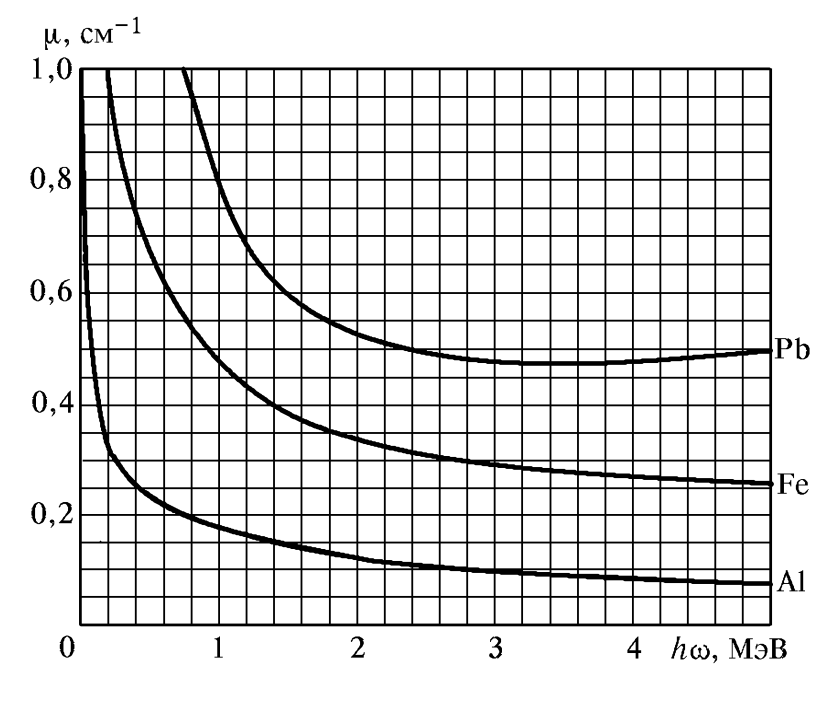
\includegraphics[width = 11 cm]{images/full_coef}
		\caption{Полные коэффициенты ослабления потока $\gamma$-лучей в алюминии, железе и свинце}
		\label{full_coef}
	\end{figure}

    В случае опытов, поставленных в хорошей геометрии, при прохождении $\gamma$-лучей через вещество меняет только количество, 
    но не энергия $\gamma$-квантов в пучке, так что коэффициент $\mu$, характеризующий поглощение $\gamma$-квантов в веществе, 
    не зависит от длины пути. Обозначим через $-dN$ число $\gamma$-квантов, выбывших их пучка на пути $dl$. 
    Это число пропорционально имеющемуся их числу $N$ и пройденному пути $dl$. Cледовательно,
    \begin{equation}
        \label{diff_eq}
        -dN = \mu N \, dl.
    \end{equation}
    Интегрируя уравнение \eqref{diff_eq} от нулевой толщины до заданной, получим
    \begin{equation}
        \label{eq3}
        N = N_0 e^{-\mu l}.
    \end{equation}

    Вообще говоря, в плохой геометрии, когда рассеянные под небольшими углами $\gamma$-кванты остаются в пучке, их спектр с прохождением вещества меняется, поэтому формула \eqref{I(mu)} неприменима. Однако в этом случае она работает лучше, чем можно было ожидать.

    Для определения коэффициента ослабления нужно, таким образом, измерить толщину образца $l$, число падающих частиц $N_0$ и число частиц $N$, прошедших через образец за фиксированное время.

\section{Экспериментальная установка}

    Схема установки, используемой в работе, показана на рис. \ref{setup1}.

    \begin{figure}[h!]
        \centering
        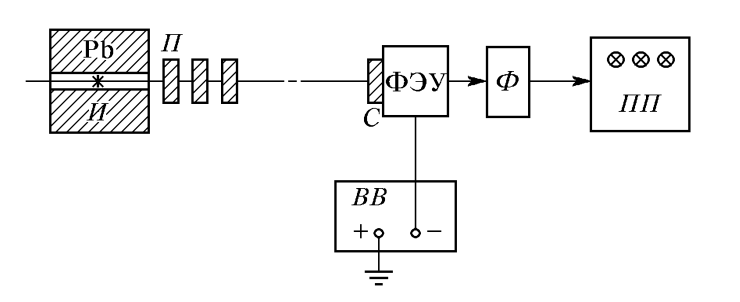
\includegraphics[width = 12 cm]{images/setup_1}
        \caption{Блок-схема установки, используемой для измерения коэффициентов ослабления коэффициентов $\gamma$-лучей: И -- источник $\gamma$-лучей; 
            Pb -- свинцовый контейнер с коллиматорным каналом; П -- набор поглотителей; С -- сцинтиллятор -- кристалл NaI(TI); Ф - формирователь-выпрямитель}
        \label{setup1}
    \end{figure}

    При недостаточно хорошей геометрии в результаты опытов могут вкрасться существенные погрешности. В установке всегда имеется конечная вероятность того, 
    что $\gamma$-квант провзаимодействует в поглотителе несколько раз до того, как попадёт в детектор (рис. \ref{setup2}). 
    Чтобы уменьшить число таких случаев, сцинтилляционный счётчик  расположен на большом расстоянии от источника $\gamma$-квантов, а поглотители имеют небольшие размеры.
    Поглотители устанавливаются на некотором расстоянии друг от друга, чтобы испытавшие комптоновское рассеяние и выбывшие из прямого потока кванты с меньшей вероятностью могли в него вернуться.

    \begin{figure}[h!]
        \begin{center}
            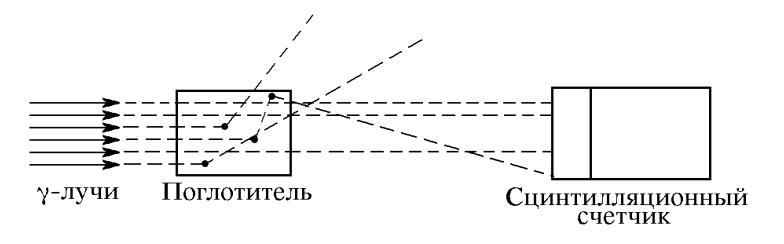
\includegraphics[width = 12 cm]{images/setup_2}
            \caption{Схема рассеяния $\gamma$-квантов в поглотителе}
            \label{setup2}
        \end{center}
    \end{figure}

\section{Ход работы}

\begin{enumerate}
    \item Включаем приборы в сеть и даём им прогреться.
    \item Подаём напряжение на ФЭУ, указанное на установке. Измеряем количество частиц при открытом и закрытом свинцовой пробкой коллиматоре. Убеждаемся, что установка <<чувствует>> $\gamma$-лучи.
    \item Измерим скорость счёта при полностью закрытом коллиматоре, так мы определим фоновое излучение. Эту скорость счёта необходимо будет вычитать для каждого измерения. 
    
        \begin{table}[h!]
            \begin{center}
            \begin{tabular}{|c|c|}
                \hline
                $N_{\text{фон}}$ & $t_{\text{фон}}$, c \\ \hline
                9720           & 300               \\ \hline
            \end{tabular}
            \caption{Измерение фонового излучения}
            \label{background}
        \end{center}
        \end{table}

    \item Измерим размеры образцов в том порядке, в котором они будут добавляться при дальнейших измерениях. 
    Измерение размеров производилось штангенциркулем с точностью $\sigma_{\ell} = 0.1 \text{ мм}$.
    
    \begin{table}[h!]
    \centering
        \begin{tabular}{|cc|cc|cc|}
            \hline
            \multicolumn{2}{|c|}{Алюминий} & \multicolumn{2}{c|}{Железо}   & \multicolumn{2}{c|}{Свинец}  \\ \hline
            \multicolumn{1}{|c|}{№}  & $\ell$, мм & \multicolumn{1}{c|}{№}  & $\ell$, мм & \multicolumn{1}{c|}{№}  & $\ell$, мм \\ \hline
            \multicolumn{1}{|c|}{1} & 19,8 & \multicolumn{1}{c|}{1} & 10,1 & \multicolumn{1}{c|}{1} & 5,2 \\ \hline
            \multicolumn{1}{|c|}{2} & 19,7 & \multicolumn{1}{c|}{2} & 10,1 & \multicolumn{1}{c|}{2} & 5,1 \\ \hline
            \multicolumn{1}{|c|}{3} & 20,0 & \multicolumn{1}{c|}{3} & 10,1 & \multicolumn{1}{c|}{3} & 5,1 \\ \hline
            \multicolumn{1}{|c|}{4} & 19,8 & \multicolumn{1}{c|}{4} & 10,2 & \multicolumn{1}{c|}{4} & 4,8 \\ \hline
            \multicolumn{1}{|c|}{5} & 20,1 & \multicolumn{1}{c|}{5} & 10,3 & \multicolumn{1}{c|}{5} & 4,8 \\ \hline
            \multicolumn{1}{|c|}{6} & 20,1 & \multicolumn{1}{c|}{6} & 10,3 & \multicolumn{1}{c|}{6} & 4,7 \\ \hline
            \multicolumn{1}{|c|}{7} & 20,4 & \multicolumn{1}{c|}{7} & 10,0 & \multicolumn{1}{c|}{7} & 4,5 \\ \hline
            \multicolumn{1}{|c|}{8} & 20,4 & \multicolumn{1}{c|}{8} & 10,2 & \multicolumn{1}{c|}{8} & 4,9 \\ \hline
            \multicolumn{1}{|c|}{9} & 20,1 & \multicolumn{1}{c|}{9} & 10,0 & \multicolumn{1}{c|}{9} & 4,5 \\ \hline
            \multicolumn{1}{|c|}{10} & 20,2  & \multicolumn{1}{c|}{10} & 10,1  & \multicolumn{1}{c|}{10} & 5,0   \\ \hline
        \end{tabular}
        \caption{Измерение размеров образцов}
        \label{sizes}
    \end{table}

    \item Теперь исследуем поглощение $\gamma$-лучей в алюминии, железе и свинце. 
    Для этого измерим число частиц, попадающих в счётчик за фиксированное время, в зависимости от общей длины поглотителя.

    \begin{table}[h!]
        \centering
        \begin{tabular}{|ccc|ccc|ccc|}
            \hline
            \multicolumn{3}{|c|}{Алюминий}                                          & \multicolumn{3}{c|}{Железо}                                            & \multicolumn{3}{c|}{Свинец}                                            \\ \hline
            \multicolumn{1}{|c|}{$N$}    & \multicolumn{1}{c|}{$t$, с} & $\ell$, мм & \multicolumn{1}{c|}{$N$}    & \multicolumn{1}{c|}{$t$, с} & $\ell$, мм & \multicolumn{1}{c|}{$N$}    & \multicolumn{1}{c|}{$t$, с} & $\ell$, мм \\ \hline
            \multicolumn{1}{|c|}{124327} & \multicolumn{1}{c|}{10}     & 0,0        & \multicolumn{1}{c|}{128362} & \multicolumn{1}{c|}{10}     & 0,0        & \multicolumn{1}{c|}{129063} & \multicolumn{1}{c|}{10}     & 0,0        \\ \hline
            \multicolumn{1}{|c|}{80321}  & \multicolumn{1}{c|}{10}     & 19,8       & \multicolumn{1}{c|}{70575}  & \multicolumn{1}{c|}{10}     & 10,1       & \multicolumn{1}{c|}{68352}  & \multicolumn{1}{c|}{10}     & 5,2        \\ \hline
            \multicolumn{1}{|c|}{54309}  & \multicolumn{1}{c|}{10}     & 39,5       & \multicolumn{1}{c|}{77065}  & \multicolumn{1}{c|}{20}     & 20,2       & \multicolumn{1}{c|}{74751}  & \multicolumn{1}{c|}{20}     & 10,3       \\ \hline
            \multicolumn{1}{|c|}{72167}  & \multicolumn{1}{c|}{20}     & 59,5       & \multicolumn{1}{c|}{64879}  & \multicolumn{1}{c|}{30}     & 30,3       & \multicolumn{1}{c|}{61643}  & \multicolumn{1}{c|}{30}     & 15,4       \\ \hline
            \multicolumn{1}{|c|}{47364}  & \multicolumn{1}{c|}{20}     & 79,3       & \multicolumn{1}{c|}{48813}  & \multicolumn{1}{c|}{40}     & 40,5       & \multicolumn{1}{c|}{49065}  & \multicolumn{1}{c|}{40}     & 20,2       \\ \hline
            \multicolumn{1}{|c|}{66416}  & \multicolumn{1}{c|}{40}     & 99,4       & \multicolumn{1}{c|}{43763}  & \multicolumn{1}{c|}{60}     & 50,8       & \multicolumn{1}{c|}{76073}  & \multicolumn{1}{c|}{100}    & 25,0       \\ \hline
            \multicolumn{1}{|c|}{45826}  & \multicolumn{1}{c|}{40}     & 119,5      & \multicolumn{1}{c|}{44308}  & \multicolumn{1}{c|}{100}    & 61,1       & \multicolumn{1}{c|}{47750}  & \multicolumn{1}{c|}{100}    & 29,7       \\ \hline
            \multicolumn{1}{|c|}{46659}  & \multicolumn{1}{c|}{60}     & 139,9      & \multicolumn{1}{c|}{55619}  & \multicolumn{1}{c|}{200}    & 71,1       & \multicolumn{1}{c|}{63663}  & \multicolumn{1}{c|}{200}    & 34,2       \\ \hline
            \multicolumn{1}{|c|}{54615}  & \multicolumn{1}{c|}{100}    & 160,3      & \multicolumn{1}{c|}{34351}  & \multicolumn{1}{c|}{200}    & 81,3       & \multicolumn{1}{c|}{40403}  & \multicolumn{1}{c|}{200}    & 39,1       \\ \hline
            \multicolumn{1}{|c|}{76022}  & \multicolumn{1}{c|}{200}    & 180,4      & \multicolumn{1}{c|}{24248}  & \multicolumn{1}{c|}{200}    & 91,3       & \multicolumn{1}{c|}{29573}  & \multicolumn{1}{c|}{200}    & 43,6       \\ \hline
            \multicolumn{1}{|c|}{55466}  & \multicolumn{1}{c|}{200}    & 200,6      & \multicolumn{1}{c|}{17862}  & \multicolumn{1}{c|}{200}    & 101,4      & \multicolumn{1}{c|}{21339}  & \multicolumn{1}{c|}{200}    & 48,6       \\ \hline
        \end{tabular}
        \caption{Измерение поглощение $\gamma$-лучей}
        \label{absorption}
    \end{table}

    \item Из теоретической зависимости ожидается экпоненциальный характер поглощения, поэтому построим соответствующие графики для трех материалов: алюминия, железа и свинца.
    
    \begin{figure}[h!]
        \centering
        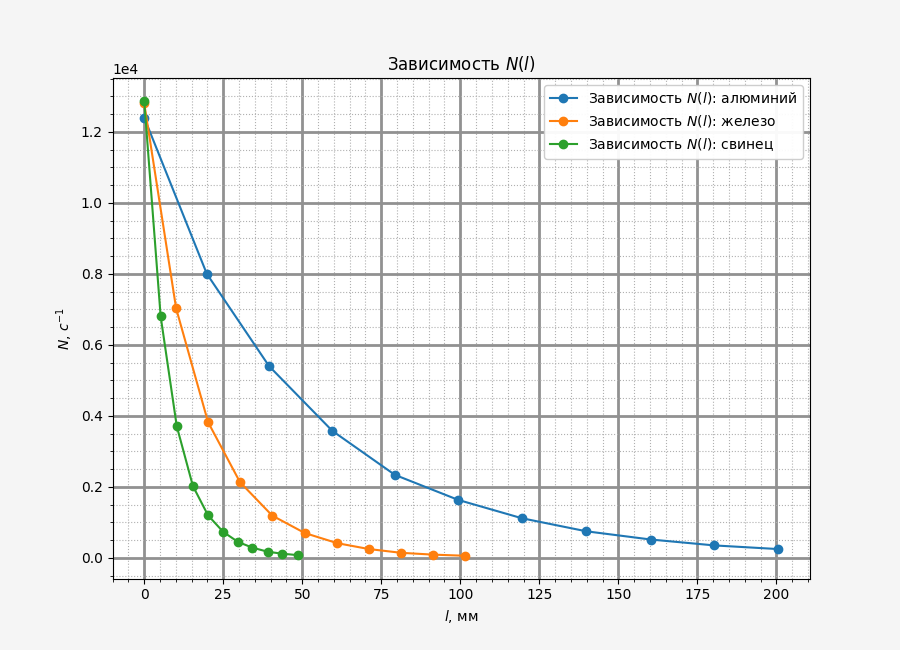
\includegraphics[width = 15 cm]{images/N_l}
        \caption{Графики зависимости $N(l)$ для алюминия, железа и свинца}
        \label{N(l)}
    \end{figure}
    
    \item Из построенных графиков в логарифмическом масштабе находим коэффициенты экспоненциальной зависимости с помощью МНК.

    \begin{figure}[h!]
        \centering
        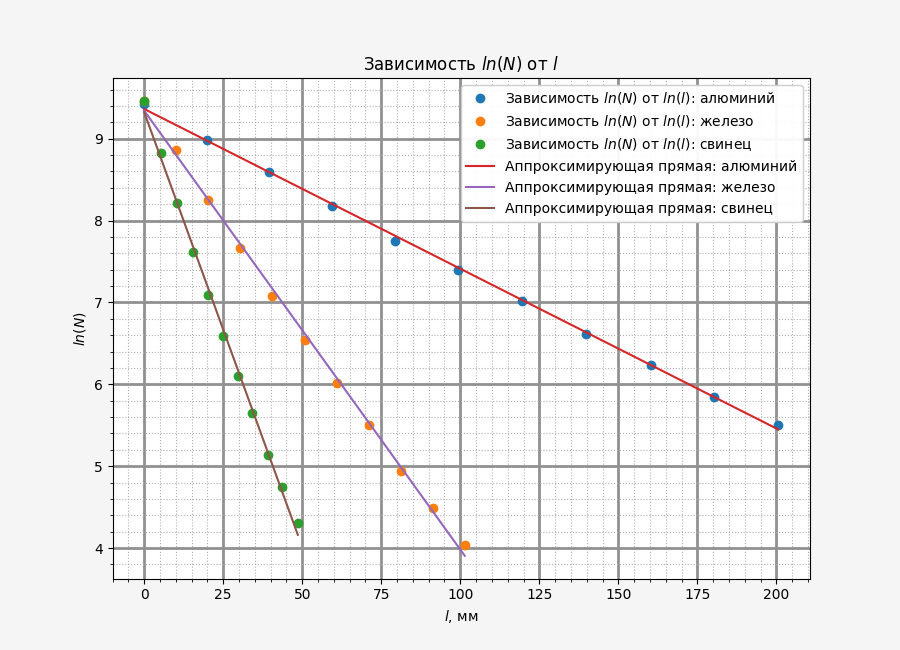
\includegraphics[width = 15 cm]{images/ln_N_l}
        \caption{Графики зависимости $N(l)$ в логарифмическом масштабе}
        \label{N(l)}
    \end{figure}
    
    \begin{table}[h!]
        \centering
        \begin{tabular}{|c|c|c|c|}
        \hline & Алюминий          & Железо            & Свинец                   \\ \hline
        $\mu$, м$^{-1}$ & $19,51 \pm 0,35$ & $53,59 \pm 1,51$ & $106,17 \pm 3,61$ \\ \hline
        \end{tabular}
        \caption{Полученные линейные коэффициенты ослабления}
    \end{table}

    \item Теперь определим другие коэффициенты ослабления из следующих соображений: 
    \[ \mu' m_1 = \mu \ell \Rightarrow \mu' = \mu \frac{\ell}{m_1} = \frac{\mu}{\rho}\]

    \begin{table}[h!]
    \centering
        \begin{tabular}{|c|c|c|c|}
        \hline & Алюминий        & Железо        & Свинец                                \\ \hline
        $\rho$,  кг/м$^3$        & 3700            & 7870          & 11350               \\ \hline
        $\mu'$, $10^{-3}$ м$^2$/кг & $5,27 \pm 0,10$ & $6,81 \pm 0,19$ & $9,35 \pm 0,32$ \\ \hline
        \end{tabular}
    \caption{Полученные линейные коэффициенты ослабления}
    \end{table}

    \item По полученным данным видим, что для всех трех материалов коэффициенты ослабления говорят о энергии $\gamma$-квантов около $0,7-0,8$ МэВ.
\end{enumerate}

\section{Определение энергии $\gamma$-квантов}

    С помощью таблицы-зависимости энергии фотона от коэффициента поглощения для различных материалов найдём энергии фотонов для всех трёх случаев (материалов): алюминий -- $E_{\gamma} = (710 \pm 20)$ КэВ, железо -- $E_{\gamma} = (750 \pm 20)$ КэВ, свинец -- $E_{\gamma} = (760 \pm 20)$ КэВ.

\section{Заключение}

    В данной работе изучено поглощения $\gamma$-лучей в трех материалах: алюминии, железе и свинце. Эксперементально определены коэффициенты поглощения материалов и соответствующие им энергии фотонов:
    \begin{table}[h!]
        \centering
        \begin{tabular}{|c|c|c|c|}
            \hline & Алюминий        & Железо        & Свинец                                \\ \hline
            $\mu$, м$^{-1}$ & $19,51 \pm 0,35$ & $53,59 \pm 1,51$ & $106,17 \pm 3,61$        \\ \hline
            $\mu'$, $10^{-3}$ м$^2$/кг & $5,27 \pm 0,10$ & $6,81 \pm 0,19$ & $9,35 \pm 0,32$ \\ \hline
            $E_{\gamma}$, КэВ & $710 \pm 20$ & $750 \pm 20$ & $760 \pm 20$ \\ \hline
        \end{tabular}
    \caption{Полученные линейные коэффициенты ослабления}
    \end{table}